\documentclass[sigconf,nonacm,natbib=false]{acmart}

\usepackage[T1]{fontenc}

\usepackage[english]{babel}

\usepackage{caption}
\usepackage{subcaption}
\usepackage{graphicx}
\graphicspath{{images/}}

\usepackage{soul}
\sethlcolor{ACMYellow}

\usepackage{tikz}
\usetikzlibrary{backgrounds,calc,fit,positioning,shapes}

\usepackage{float}

\usepackage[all]{nowidow}

\usepackage[backend=biber,style=ACM-Reference-Format,sorting=none]{biblatex}
\addbibresource{final-paper.bib}

\usepackage{csquotes}
\SetCiteCommand{\autocite}

\usepackage{listings}
\lstdefinelanguage{json}{
  basicstyle=\small\ttfamily,
  breakindent=4.8ex,
  basewidth=0.55em,
  showstringspaces=false,
  morestring=[b]",
  stringstyle=\color{ACMRed},
  keywords=[0]{true,false},
  keywordstyle=[0]\color{ACMPurple},
  literate=
    *
    {0}{{{\color{ACMBlue}0}}}{1}
    {1}{{{\color{ACMBlue}1}}}{1}
    {2}{{{\color{ACMBlue}2}}}{1}
    {3}{{{\color{ACMBlue}3}}}{1}
    {4}{{{\color{ACMBlue}4}}}{1}
    {5}{{{\color{ACMBlue}5}}}{1}
    {6}{{{\color{ACMBlue}6}}}{1}
    {7}{{{\color{ACMBlue}7}}}{1}
    {8}{{{\color{ACMBlue}8}}}{1}
    {9}{{{\color{ACMBlue}9}}}{1}
    {:}{{{\color{ACMDarkBlue}{:}}}}{1}
    {,}{{{\color{ACMDarkBlue}{,}}}}{1}
    {\{}{{{\color{ACMDarkBlue}{\{}}}}{1}
    {\}}{{{\color{ACMDarkBlue}{\}}}}}{1}
    {[}{{{\color{ACMDarkBlue}{[}}}}{1}
    {]}{{{\color{ACMDarkBlue}{]}}}}{1},
}
\lstdefinelanguage{turtle}{
  basicstyle=\small\ttfamily,
  breakindent=4.8ex,
  basewidth=0.55em,
  showstringspaces=false,
  morecomment=[l]{\#},
  commentstyle=\color{gray},
  morestring=[b]",
  morestring=[s]{<}{>},
  stringstyle=\color{ACMRed},
  classoffset=0,
  morekeywords={owl,rdf,xml,xsd,rdfs,saref,s4envi,ssn,geo,td,om},
  keywordstyle=\color{ACMBlue},
  classoffset=1,
  morekeywords={@prefix,@base,@en},
  keywordstyle=\color{ACMOrange},
  classoffset=0,
  literate=
    *
    {:}{{{\color{ACMBlue}{:}}}}{1}
    {;}{{{\color{ACMDarkBlue}{;}}}}{1}
    {,}{{{\color{ACMDarkBlue}{,}}}}{1}
    {.}{{{\color{ACMDarkBlue}{.}}}}{1}
    {[}{{{\color{ACMDarkBlue}{[}}}}{1}
    {]}{{{\color{ACMDarkBlue}{]}}}}{1},
}
\lstdefinelanguage{jsonpath}{
  basicstyle=\small\ttfamily,
  breakindent=4.8ex,
  basewidth=0.55em,
}

\lstset{
  basicstyle=\ttfamily,
  frame=lines,
  breaklines=true,
}

\usepackage{bookmark}
\bookmarksetup{numbered,open}

\usepackage[nonumberlist,automake]{glossaries-extra}
\makeglossaries{}
\setabbreviationstyle{short-nolong}
\setabbreviationstyle[acronym]{long-short}
\setglossarystyle{list}
\loadglsentries{glossary}

\begin{document}

\title{Extending the Web of Things to standardize Service Discovery in Smart Cities}

\author{Tristan Damm}
\affiliation{%
  \institution{Hochschule Flensburg}
  \streetaddress{Kanzleistraße 91--93}
  \city{Flensburg}
  \country{Germany}
  \postcode{24943}
}
\email{tristan.damm@stud.hs-flensburg.de}

\author{Ellen Landschoof}
\affiliation{%
  \institution{Hochschule Flensburg}
  \streetaddress{Kanzleistraße 91--93}
  \city{Flensburg}
  \country{Germany}
  \postcode{24943}
}
\email{ellen.landschoof@stud.hs-flensburg.de}

\author{Lukas Obermann}
\affiliation{%
  \institution{Hochschule Flensburg}
  \streetaddress{Kanzleistraße 91--93}
  \city{Flensburg}
  \country{Germany}
  \postcode{24943}
}
\email{lukas.obermann@stud.hs-flensburg.de}

\author{Louis Richter}
\affiliation{%
  \institution{Hochschule Flensburg}
  \streetaddress{Kanzleistraße 91--93}
  \city{Flensburg}
  \country{Germany}
  \postcode{24943}
}
\email{louis.richter@stud.hs-flensburg.de}

\author{Tjorben Wade}
\affiliation{%
  \institution{Hochschule Flensburg}
  \streetaddress{Kanzleistraße 91--93}
  \city{Flensburg}
  \country{Germany}
  \postcode{24943}
}
\email{tjorben.wade@stud.hs-flensburg.de}

\keywords{Open Data, Service Discovery, Smart City, Web of Things}

\renewcommand{\shortauthors}{Damm and Landschoof, et al.}

\begin{abstract}
% Purpose
European member states are required to make collected data from sensors available to the public while not imposing any standard on the format and scope of the provided information. This greatly decreases the discoverability and usability of that data for developers and thus the public. In this paper, we propose a new solution by creating a standard ontology for the \glsfirst{wot} standard.

% Method/Findings
To evaluate our approach, a reference implementation was built, consisting of a \glsfirst{tdd} and a showcasing real-life client. Our tests verified the approach as successful, while revealing potential problems and difficulties of the \glsfirst{jsonld} format.

% Originality/Value
This paper provides the approach for handling open data in a uniform way, while being easily extendable for new use cases. It thus serves as a foundation for standardization work and further research on this topic.

\end{abstract}

\maketitle

% \section{Einleitung}

% Dies ist eine Einleitung.

% \begin{itemize}
%   \item List item
%   \item Test
% \end{itemize}

% \begin{enumerate}
%   \item test
% \end{enumerate}

% \enquote{Dies ist ein Zitat.} \autocites[vgl.][]{Apple.HIG}{Apple.HIG}.

% \autocite[vgl.][]{GermanConventionBureau.2021.DKaSbViDvunCpB}

% \textcquote[vgl.][]{Apple.HIG}{Individualisten, mit dem Ziel der persönlichen Einkommens- und Lebenslustmaximierung}

% \subsection{Sub }

% \subsubsection{Sub}

\section{Introduction}\label{sec:introduction}

The deployment of \gls{iot} devices and sensors in cities has increased significantly in recent years, and these systems play a crucial role in collecting data that provides various information about the environment.
For example, sensors can measure the current temperature in the city center, or help a driver locate unused parking spots in the city center.
In this paper, we investigate the development of a \gls{wot} solution for the standardization of \gls{iot} systems interfaces used by cities.

The problem is that the interfaces of these sensors are not consistent, making it difficult for developers to access the data.
A European directive \autocite{digital-strategy.ec.europa.eu} requires member states, among other things, to make the data collected by sensors available to the public, but they have the freedom to decide how to do so.
This means that each city can use its own standards, which complicates interoperability. This makes it difficult for developers to create applications that can use data from multiple sources.
Therefore, it is necessary to find a solution that allows data from different sources to be combined and a standard format to be set.

The authors of this paper previously conducted a study titled \citetitle{Survey.Service.Discovery.in.Smart.Cities} \autocite{Survey.Service.Discovery.in.Smart.Cities} in which various solutions were examined.
In this study, the \gls{wot} technology emerged as the best solution. It is used to extend the functionality of \gls{iot} and optimize \gls{sd}.

The goal of this study was to develop an extended \gls{wot} solution that allows cities to combine and make data from different \gls{iot} systems accessible.
Furthermore, it will be demonstrated using a test environment that the solution can be successfully implemented and utilized.

As part of this paper, a backend system was developed to store and manage sensor information.
The backend system uses a format that is based on \gls{wot} and has been extended by us.
It allows for the integration and processing of data from various sensors and devices.
Additionally, a mobile application was created as a frontend system that works with sensor data to test the backend.
This application demonstrates how developers can use data from the backend to create applications that work with sensor data.
In our example, the application can be used to display temperatures at different locations.

We have shown that it is possible to develop a backend that uses this new standard and that it is possible to create applications that can work with this data.
We believe that the development of an extended \gls{wot} solution for the standardization of \gls{iot} systems interfaces will greatly benefit cities and developers by providing a unified and easily accessible data source.

Initially, important fundamentals will be explained, in order to subsequently delve into the relevant problem.
Later on, the solution will be presented and the structure of the corresponding test environment will be explained.
Afterwards, we will discuss the work and draw a conclusion.

\section{Related Work}\label{sec:relatedworks}

One of the main aspects of our research were different \glspl{sd}. We concentrated on three most suited for our work.

\subsection{Semantic \glsentrylong{sd}}\label{sec:semanticsd}

The main aspect of semantic \gls{sd} is to find services based on an ontology. An ontology is a way of describing how different properties are related to each other. They are used to build a shared vocabulary and unambiguous meaning across a subject area.
While many other \glspl{sd} only work with functional properties (e.g. accepted message types, required inputs, \dots), semantic \gls{sd} uses functional and non-functional (e.g. performance, cost, reliability, \dots) properties alike.

How a semantic \gls{sd} is structured is highly dependent on the purpose it was built for and who it was built by. Since there is no standardization in place the discovery process as well as the used ontology can be adjusted to fit the developer's needs. This makes it possible for \citeauthor{Iqbal.12320081252008.SSDuSaS} \autocite{Iqbal.12320081252008.SSDuSaS} to describe services using \emph{SAWSDL} and \emph{SPARQL} while \citeauthor{BenMokhtar.2006.ESSDiPCE} \autocite{BenMokhtar.2006.ESSDiPCE} use \emph{Amigo-S} and \emph{S-Ariadne} in their work. There are also a lot of different approaches on how to select suitable services for users \autocite{Majithia.2004.Rbssd} \autocite{Jia.2017} \autocite{Zhao.2017}.

\subsection{Quality-of-Service-based \glsentrylong{sd}}\label{sec:qossd}

\glsdisp{qos}{Quality-of-Service-based (\glsxtrshort{qos})} \glspl{sd} are focused on non-functional evaluation criteria. The \gls{qos} aspect includes all measures over the quality of a communication service from the user's point of view (e.g. bandwidth, latency, transmission rate, \dots). \glsxtrshort{qos}-based \glspl{sd} can be divided into subcategories \autocite{Achir.2020.AtosdaiI}:

\begin{itemize}
\item Security-based
\item Energy-consumption-based
\item Network-infrastructure-based
\end{itemize}

Additionally, there are hybrid categories which can include a combination of two or all other categories.

The security-based aspect can be omitted for our work since we will be working with open data. Energy consumption and network infrastructure are considerably more important since most sensors have restricted resources.

In most cases, \glsxtrshort{qos}-based \glspl{sd} are based on other \gls{sd} approaches like semantic \gls{sd}. This makes them quite versatile. While the base \gls{sd} works just like it always does. After a service was found, the \glsxtrshort{qos}-based \gls{sd} acts as a kind of \gls{qos} filter \autocite{Kosunalp.2020.SArlbQaIsdm}. Thereby services that are not suitable get rejected.

One example of \glsxtrshort{qos}-based \gls{sd} is the concept of \emph{SARL}, which is based on a peer-to-peer concept that by itself does not cover \gls{qos} factors.

\subsection{Context-based Service discovery}\label{sec:contextsd}

Another \gls{sd} is the context-based \gls{sd}.

\textcquote{Sukode.2015.CAFIIAS}{Context is any information that can be used to characterize the situation of an entity. An entity is a person, place, or object that is considered relevant to the interaction between a user and an application, including the user and applications themselves.}

A context like that can be defined and used to describe different services. Each area of use can be defined by a different context. How that context is built and structured depends on the usage.

If a system takes a context into account, it is called \enquote*{context-aware}. It can be used to locate the best possible service for a user.

\subsection{\glsentrylong{wot}}\label{sec:wot}

One problem with \gls{sd} in the \gls{iot} space is always interoperability and compatibility between different systems. One area where these aspects are highly relevant is the internet. Web technologies must work for a wide range of devices and applications. Thus, the internet has also been used as a source of inspiration for solving such and other problems with \gls{iot} devices. This combination is commonly referred to as \gls{wot}, which we examined in a previous survey paper \autocite{Survey.Service.Discovery.in.Smart.Cities}.

The \gls{wot} offers a standard that covers the description of sensors as well as the implementation of \gls{sd}. These descriptions are kept up-to-date and are very comprehensive compared to the \gls{sd} structures examined. However, In some places the standard is not yet fully developed.

Another survey paper about the \gls{wot} by \citeauthor{Sciullo.2022.ASotWoT} \autocite{Sciullo.2022.ASotWoT} covers various aspects of the specification such as architecture, communication protocols, security, and applications. It also covers challenges and future directions of \gls{wot} research.


\section{State of the Art}\label{sec:stateoftheart}

\subsection{Thing Description}\label{sec:thingdescription}

\gls{td} is a \gls{w3c} standard to describe \gls{iot} devices and their properties. Developers can use them to describe devices in a clear and standardized way. The description can be used in applications or services to know how to interact with a device.
A \gls{td} contains different properties and types. These include the type of device, available features or data, used protocols and the type of data a device is providing.
An application using data from this device (e.g. the app discussed in this paper) should be able to read this standard and extract the needed information. \glspl{td} are written in \gls{json} and use the \gls{jsonld} standard to provide the information.

A \gls{td} uses different vocabularies to define properties and types. The basic structure is defined by a core vocabulary. This contains a root object called \emph{Thing}. A \emph{Thing} object provides a \gls{uri},
labels and metadata. In order to interact with a \emph{Thing}, it additionally provides \emph{Interaction Affordances}. There are three types of \emph{Interaction Affordances}:
\begin{itemize}
  \item \emph{Property Affordances}
  \item \emph{Action Affordances}
  \item \emph{Event Affordances}
\end{itemize}

A \emph{Property Affordance} describes where you can get information provided by the device. As in the example discussed in this paper, this could be the measured values of a sensor.
An \emph{Action Affordance} describes how to interact with the device. It should define what the input and output data should look like.
An \emph{Event Affordance} describes an interface where you will be notified of new information. It defines the data to subscribe or unsubscribe from an event.

\begin{lstlisting}[language=json,caption={Example for a \gls{td}},label={lst:example-td}]
{
  "@context": [
    "https://www.w3.org/2022/wot/td/v1.1",
    {
      "sdsc": "https://sdsc.fly.dev/ontology#",
      "ssn": "http://www.w3.org/ns/ssn/",
      "om": "http://www.ontology-of-units-.../om-2/",
      "om18": "http://www.wurvoc.org/.../om-1.8/",
      "geo": "http://www.w3.org/.../wgs84_pos#",
      "saref": "https://saref.etsi.org/core/",
      "s4envi": "https://saref.etsi.org/saref4envi/",
      "time": "http://www.w3.org/2006/time#"
    }
  ],
  "@type": "sdsc:TemperatureSensor",
  "id": "https://hansen.de/temperature/1",
  "title": "Measuring station Hansen",
  "geo:lat": 54.789401,
  "geo:long": 9.416152,
  "s4envi:hasFrequencyMeasurement": {
    "@type": "s4envi:FrequencyMeasurement",
    "saref:isMeasuredIn": {
      "@id": "om18:reciprocal_hour"
    },
    "saref:hasValue": 1
  },
  "s4envi:hasTransmissionPeriod": {
    "@type": "s4envi:PeriodMeasurement",
    "saref:isMeasuredIn": {
      "@id": "time:unitSecond"
    },
    "saref:hasValue": 5
  },
  "saref:measuresProperty": {
    "@id": "sdsc:Temperature"
  },
  "securityDefinitions": {
    "opendata": {
      "scheme": "nosec"
    }
  },
  "security": ["opendata"],
  "properties": {
    "temperature": {
      "@type": "sdsc:TemperatureAffordance",
      "ssn:forProperty": {
        "@id": "sdsc:Temperature"
      },
      "type": "number",
      "unit": "om:degreeCelsius",
      "readOnly": true,
      "forms": [
        {
          "href": "https://.../temperature",
          "op": "readproperty"
        }
      ]
    }
  }
}
\end{lstlisting}

\autoref{lst:example-td} presents an example of a \gls{td} defined for a temperature sensor. The type of the sensor is defined by the \lstinline|@type| property. In this project, two sensor types were defined.

The \lstinline|sdsc:TemperatureSensor| defines a temperature sensor, while \lstinline|sdsc:WindSpeedSensor| defines sensors for measuring wind speed.

The \lstinline|id|-field must contain a unique identifier for the sensor. We are using the \gls{uri} of thing to identify the sensor. The \lstinline|title| can be defined by the owner of a sensor. It should contain a name that helps the user understand what the sensor does and where it is located.

Additionally, we added two new fields to the \gls{td}['s] vocabulary to offer the opportunity to set location data. This means that fields \lstinline|geo:lat| and \lstinline|geo:long| must be included in the \gls{td} in order to provide latitude and longitude for a sensor.

The \lstinline|s4envi:hasFrequencyMeasurement| field provides information about the time between measurements. It contains a unit in which the duration is measured and the value. A similar field is \lstinline|s4envi:hasTransmissionPeriod|. This field provides information about the duration of a transmission from the sensor to the server. It contains fields for the value and the unit. Both fields also do not appear in the standard vocabulary.

The \gls{wot} standard specifies \lstinline|securityDefinitions| and its accompanying \lstinline|security| field to provide data about authentication when accessing a sensor. A public API for fetching data in a smart city was planned. For this reason, a security scheme for open data with no authentication at the server was defined.

The \gls{td} shown in \autoref{lst:example-td} contains only one Interaction Affordance. It does not need Action Affordances, because the sensor does not provide an opportunity to change any settings, and Event Affordances, because the sensor does not send any events. The \lstinline|properties| field contains Property Affordances for temperature or wind speed. It specifies a unit (degrees in this case) and the form from which one can get the actual value for this property.

\subsection{\glsentrytext{jsonld}}\label{sec:jsonldinfo}

\gls{jsonld} is the format used throughout the \gls{wot}, with its main use being \glspl{td}. It adds a semantic layer to a \gls{json} structure to let every property be a globally unique identifier -- a \gls{uri} -- based on ontologies. \gls{jsonld} provides different ways how to represent data. The most common way is to provide a so-called \enquote*{context}, so you can use more readable property names for the actual data. The context is a nested \gls{json} structure that maps the property names to the actual identifiers. \autoref{lst:example-td} shows an exemplary \gls{td} document, where the \gls{wot} ontology \cite{w3c.wot.tdo.20230111} and other secondary ontologies are referenced in its context. Some \glspl{uri} have been abbreviated for formatting reasons.

Property names use terms from a referenced context document, which provides a description and \gls{uri} for the property. Auxiliary ontologies may be referred to using a prefix. The process of getting the actual structure and identifiers is called \enquote{expansion}. Its result is a \gls{json} document where each property is a \gls{uri}. Due to the flexible nature of how to reference ontologies, two documents with the exact same semantic meaning may not have equal \gls{jsonld} representations, i.e. they're not structurally equal. Only if documents are fully expanded, they are structurally comparable (excluding arrays where the order does not matter). \autoref{lst:example-jsonld-document-expanded} shows an excerpt of the expanded example \gls{td} document from \autoref{lst:example-td}, which is -- at least seemingly -- larger, due to the \gls{uri} expansion, and deeper nested.

\begin{lstlisting}[language=json,caption={Example \gls{jsonld} document expanded},label={lst:example-jsonld-document-expanded}]
[
  {
    "@type": [
      "https://...fly.dev/ontology#TemperatureSensor"
    ],
    "@id": "https://example.com/temperature/1",
    "https://www.w3.org/2019/wot/td#title": [
      {
        "@value": "Nowhere Temperature Sensor"
      }
    ],
    ...
    "https://.../td#hasPropertyAffordance": [
      {
        "@type": [
          "https://...ntology#TemperatureAffordance",
          "https://.../wot/json-schema#NumberSchema"
        ],
        "https://.../wot/td#hasForm": [
          {
            "https://.../wot/hypermedia#hasTarget": [
              {
                "@value": "https://.../temperature"
              }
            ],
            ...
          }
        ],
        ...
      }
    ]
  }
]
\end{lstlisting}


\section{Problem Statement}\label{sec:problem-statement}

The data published by cities does not have a uniform format, with both structured formats such as \gls{json} and unstructured formats such as plain text being used, which makes automated processing of the data more difficult \autocite{govdata}. Currently, there is no comprehensive solution to this problem, as existing systems only provide partial solutions or are not specific enough for the Smart City sensor application domain.

Determining whether the \gls{wot} and its associated \glspl{td} are a good solution is part of our problem, as so far it appears to be the best approach, providing structure and semantic expressiveness for this use case. However, the \gls{wot} does not make assumptions about the content of descriptions and ontologies used for Smart City applications are neither standardized nor provide a common vocabulary that covers a wide range of Smart City sensor application domains. Additionally, the \gls{wot} does not include \gls{qos} aspects, which can be important for \gls{sd}, enhancing the quality and preciseness of search.

In order to enable search, the \gls{wot} provides different search type options that may be implemented \autocite[section 7.3.2.3]{w3c.wot.discovery.20210602}. It is to be validated that at least of these search options is suitable for \gls{sd} of public sensors.

A challenge is to extend the \gls{wot} to solve all the mentioned problems. Additionally, it must also be tested in practice to check for its functionality. In \autoref{sec:pocapplication}, the implementation of a proof of concept is examined, and it is shown how this solution can be used in a test environment.

\section{Proof-of-Concept Application}\label{sec:pocapplication}

\subsection{Ontology}\label{sec:ontology}

To overcome this problem, we propose a new ontology that is based on already established ontologies and aligns with the \citetitle{w3c.wot.tdo.20230111} for specific use in \glspl{td} and, at the same time, an easy way to extend the ontology if new application areas are needed.

The core element of the ontology is the \lstinline|Sensor| class, which is built on top of the \lstinline|Sensor| class from \citetitle{etsi.saref.core} and its extensions from the \citetitle{etsi.saref.envi}. Also inheriting properties from the \citetitle{w3c.geo}, the \lstinline|Sensor| class provides important \gls{qos} features such as the location, measurement frequency and data transmission period. The class is intended to be sub-classed for each sensor type to have a common set of important values available to retrieve independent of the sensor type.

Each sensor type consists of a set of different classes and named individuals, as seen in \autoref{fig:ontology-parts-per-sensor-type}. This includes the parts which are the same across all sensor types, which makes it easy to extend the ontology with new sensor types.

\begin{figure}[H]
  \begin{tikzpicture}[
    node distance=30mm and 15mm,
    on grid,
    text height=1.5ex, % size including ascenders
    text depth=.1ex,   % descenders size
    class/.style={
      draw=ACMPurple,
      inner xsep=6pt,
      inner ysep=6pt,
      rectangle,
      draw,
      line width=1pt,
    },
    namedindividual/.style={
      draw=ACMOrange,
      inner xsep=6pt,
      inner ysep=6pt,
      rounded rectangle,
      draw,
      line width=1pt,
    },
    edgedesc/.style={
      font=\ttfamily\scriptsize,
    },
  ]
    \node (s) [class] {Sensor};
    \node (pa) [class,below right=of s,xshift=10mm] {Property Affordance}
      edge [<-] node [edgedesc,above,sloped,xshift=1mm] {td:hasPropertyAffordance} (s);
    \node (p) [class,below left=of pa] {Property}
      edge [<-] node [edgedesc,below,sloped,yshift=2pt] {saref:measuresProperty} (s)
      edge [<-] node [edgedesc,above,sloped]            {ssn:forProperty}        (pa);
    \node (pu) [class,below=of p,xshift=-5mm,yshift=10mm] {Property Unit}
      edge [<-] node [edgedesc,right] {om:commonlyHasUnit} (p);
    \node (u1) [namedindividual,below left=of pu,yshift=10mm] {Unit 1}
      edge [->] node [edgedesc,above,sloped,xshift=-1mm] {rdf:type} (pu);
    \node (u2) [namedindividual,below=of pu,yshift=10mm] {Unit 2}
      edge [->] node [edgedesc,above,sloped] {rdf:type} (pu);
    \node (u2) [namedindividual,below right=of pu,yshift=10mm] {…}
      edge [->] node [edgedesc,above,sloped,xshift=1mm] {rdf:type} (pu);
    \node (m) [class,below left=of s,xshift=-10mm] {Measurement}
      edge [->] node [edgedesc,above,sloped,xshift=-1mm]  {saref:measurementMadeBy} (s)
      edge [->] node [edgedesc,above,sloped,xshift=1.5mm] {saref:relatesToProperty} (p)
      edge [->] node [edgedesc,below,sloped,yshift=1pt]   {saref:isMeasuredIn}      (pu);
  \end{tikzpicture}
  \caption{Ontology parts for each sensor type}\label{fig:ontology-parts-per-sensor-type}
\end{figure}

The class that subclasses \lstinline|Sensor| represents the root of the \gls{td}. The \lstinline|Measurement| is not a direct part of the \gls{td}, which is defined by the other parts mentioned in \autoref{fig:ontology-parts-per-sensor-type}, but serves as the definition of the format used to serve the data of a single measurement. This ensures a unified data format for all sensors of a type. The \lstinline|Property| mainly serves as a description of the actual property to measure and to bind the property's unit classes. The \lstinline|Property Unit| is only used to provide a common type for all named individuals that represent each possible unit of the property.

We applied this principle to multiple measurable values to verify it works for different use cases. Hereafter, we will discuss one of those examples in detail.

Our ontology is defined using Turtle syntax \autocite{w3c.turtle}, since most of the existing ontologies are also defined using this syntax. To fully understand our ontology, we first introduce the used prefixes and their expanded \gls{uri} forms in \autoref{lst:ontology-prefixes}.

\begin{lstlisting}[language=turtle,caption={Ontology prefixes},label={lst:ontology-prefixes}]
@prefix : <https://sdsc.fly.dev/ontology#> .
@prefix owl: <http://www.w3.org/2002/07/owl#> .
@prefix rdf: <http://www.w3.org/1999/02/22-rdf-syntax-ns#> .
@prefix xml: <http://www.w3.org/XML/1998/namespace> .
@prefix xsd: <http://www.w3.org/2001/XMLSchema#> .
@prefix rdfs: <http://www.w3.org/2000/01/rdf-schema#> .
@prefix saref: <https://saref.etsi.org/core/> .
@prefix s4envi: <https://saref.etsi.org/saref4envi/> .
@prefix ssn: <http://www.w3.org/ns/ssn/> .
@prefix geo: <http://www.w3.org/2003/01/geo/wgs84_pos#> .
@prefix td: <https://www.w3.org/2019/wot/td#> .
@prefix om: <http://www.ontology-of-units-of-measure.org/resource/om-2/> .
@base <https://sdsc.fly.dev/ontology> .
\end{lstlisting}

The \lstinline|Sensor| class is the core class (\autoref{lst:sensor-class}). It is only defined once and is sub-classed by \lstinline|TemperatureSensor|, which is our example sensor type and on which its measured property and the temperature affordance for the \gls{td} are defined (\autoref{lst:temperaturesensor-class}). The \lstinline|Sensor| class also makes it possible to include \gls{qos} aspects like location, the frequency of measurements and the transmission period.

\begin{lstlisting}[language=turtle,caption={{\ttfamily{}Sensor} class},label={lst:sensor-class}]
###  https://sdsc.fly.dev/ontology#Sensor
:Sensor
  rdf:type owl:Class ;
  rdfs:subClassOf
    geo:SpatialThing ,
    saref:Sensor ,
    [ rdf:type owl:Restriction ;
      owl:onProperty s4envi:hasFrequencyMeasurement ;
      owl:allValuesFrom s4envi:FrequencyMeasurement
    ] ,
    [ rdf:type owl:Restriction ;
      owl:onProperty s4envi:hasTransmissionPeriod ;
      owl:allValuesFrom s4envi:PeriodMeasurement
    ] .
\end{lstlisting}

\begin{lstlisting}[language=turtle,caption={{\ttfamily{}TemperatureSensor} class},label={lst:temperaturesensor-class}]
###  https://sdsc.fly.dev/ontology#TemperatureSensor
:TemperatureSensor
  rdf:type owl:Class ;
  rdfs:subClassOf
    :Sensor ,
    [ rdf:type owl:Restriction ;
      owl:onProperty saref:measuresProperty ;
      owl:someValuesFrom :Temperature
    ] ,
    [ rdf:type owl:Restriction ;
      owl:onProperty td:hasPropertyAffordance ;
      owl:someValuesFrom :TemperatureAffordance
    ] .
\end{lstlisting}

The \lstinline|TemperatureAffordance| class then restricts the permitted values for its property affordance to \lstinline|Temperature| values (\autoref{lst:temperatureaffordance-class}).

\begin{lstlisting}[language=turtle,caption={{\ttfamily{}TemperatureAffordance} class},label={lst:temperatureaffordance-class}]
###  https://sdsc.fly.dev/ontology#TemperatureAffordance
:TemperatureAffordance
  rdf:type owl:Class ;
  rdfs:subClassOf
    [ rdf:type owl:Restriction ;
      owl:onProperty ssn:forProperty ;
      owl:someValuesFrom :Temperature
    ] .
\end{lstlisting}

A \lstinline|Temperature| is defined by a common unit and can be labelled and described (\autoref{lst:temperature-class}). The associated \lstinline|TemperatureUnit| is defined as a class, which each of its actual units as named individuals (\autoref{lst:temperatureunit-class}). Those individuals are imported from another ontology and mapped onto the \lstinline|TemperatureUnit| class.

\begin{lstlisting}[language=turtle,caption={{\ttfamily{}Temperature} class},label={lst:temperature-class}]
###  https://sdsc.fly.dev/ontology#Temperature
:Temperature
  rdf:type owl:Class ;
  rdfs:subClassOf saref:Property ;
  om:commonlyHasUnit :TemperatureUnit ;
  rdfs:comment "Temperature is the extent to which an object is hot."@en ;
  rdfs:label "Temperature"@en .
\end{lstlisting}

\begin{lstlisting}[language=turtle,caption={{\ttfamily{}TemperatureUnit} class and its named individual(s)},label={lst:temperatureunit-class}]
###  https://sdsc.fly.dev/ontology#TemperatureUnit
:TemperatureUnit rdf:type owl:Class ;
  rdfs:subClassOf
    om:Unit ,
    saref:UnitOfMeasure ;
  rdfs:comment "The unit of measure for temperature"@en ;
  rdfs:label "Temperature unit"@en .

###  http://www.ontology-of-units-of-measure.org/resource/om-2/degreeCelsius
om:degreeCelsius
  rdf:type
    owl:NamedIndividual ,
    :TemperatureUnit .
\end{lstlisting}

The \lstinline|TemperatureMeasurement| class connects the different parts by referencing the sensor class, the property, its unit and the format, in which the measurement is made (\autoref{lst:temperaturemeasurement-class}).

\begin{lstlisting}[language=turtle,caption={{\ttfamily{}TemperatureMeasurement} class},label={lst:temperaturemeasurement-class}]
###  https://sdsc.fly.dev/ontology#TemperatureMeasurement
:TemperatureMeasurement
  rdf:type owl:Class ;
  rdfs:subClassOf
    saref:Measurement ,
    [ rdf:type owl:Restriction ;
      owl:onProperty saref:measurementMadeBy ;
      owl:someValuesFrom :TemperatureSensor
    ] ,
    [ rdf:type owl:Restriction ;
      owl:onProperty saref:relatesToProperty ;
      owl:someValuesFrom :Temperature
    ] ,
    [ rdf:type owl:Restriction ;
      owl:onProperty saref:isMeasuredIn ;
      owl:someValuesFrom :TemperatureUnit
    ] ,
    [ rdf:type owl:Restriction ;
      owl:onProperty saref:hasValue ;
      owl:allValuesFrom xsd:float
    ] .
\end{lstlisting}

\subsection{Backend}\label{sec:backend}

The \gls{wot} only provides the specification for a \gls{tdd} service \autocite[section 7.3]{w3c.wot.discovery.20210602}, but there are no full implementations of the standard yet. Therefore, we implemented the relevant parts of the Thing Description Directory specification.

A centralized service is necessary for identifying and accessing the \glspl{td} provided by multiple sources. The \gls{td} will be obtained through a single \gls{url} that leads to a provider service, which returns the \gls{td} metadata. The service caches the \gls{td} metadata in a database for efficient retrieval and provides an \gls{api} for accessing it. Additionally, the service keeps track of the respective providers for each \gls{td} and allows them to register and manage their own \glspl{td}, as well as store additional information about the providers themselves. Furthermore, the implementation of the service follows the \gls{tdd} guidelines specified by the \gls{wot}.

A \gls{sd} process starts with a request being sent to a thing provider, which returns the \gls{td} metadata. This is stored in a database along with other associated data such as the provider itself. A client can then retrieve one or more \glspl{td} via the \gls{api}.

\subsubsection{API}\label{sec:apibackend}

The \gls{api} is a trimmed down implementation of the \gls{wot} Directory Service \gls{api} and is responsible for retrieving, listing and searching \glspl{td}, while also offering an Events \gls{api} to notify clients about the changes to \glspl{td}. The ontology described earlier in this paper is provided over a separate endpoint.

The following list shows all openly accessible endpoints to the clients:

\begin{itemize}
    \item \lstinline|/ontology| shows our defined ontology.
    \item \lstinline|/api/things| returns a paginated list of \glspl{td}.
    \item \lstinline|/api/things/{id}| returns a single \gls{td}, where the \lstinline|id| parameter is the \gls{uri} of the \gls{td}.
    \item \lstinline|/api/search/jsonpath?query={query}| searches \glspl{td} with an \emph{JSONPath} expression as the query parameter.
    \item \lstinline|/events/{type}| informs about changes to \glspl{td} via \gls{SSE} where the type specifies the event.
\end{itemize}

\subsubsection{Admin-Panel}\label{sec:adminpanel}

The administration panel is a web app that manages the data of the \gls{tdd} as well as information about the organizations that provide \gls{td} metadata. Organizations administrators can register new \glspl{td} and edit their organization information.


\subsection{Frontend}\label{sec:frontend}

We developed an Android application to utilize our \gls{api} as outlined in the introduction. The app serves as a reference implementation for connecting the backend functions shown in \autoref{sec:backend}.

The following requirements were defined by us in advance:

\begin{itemize}
    \item Filter for geographic location and a radius, minimal frequency of measurements (\gls{qos} aspects)
    \item Quick overview of the sensors in a smart city (around location)
    \item Capability to display sensors metadata and the measured values
\end{itemize}

\begin{figure}[H]
    \centering
    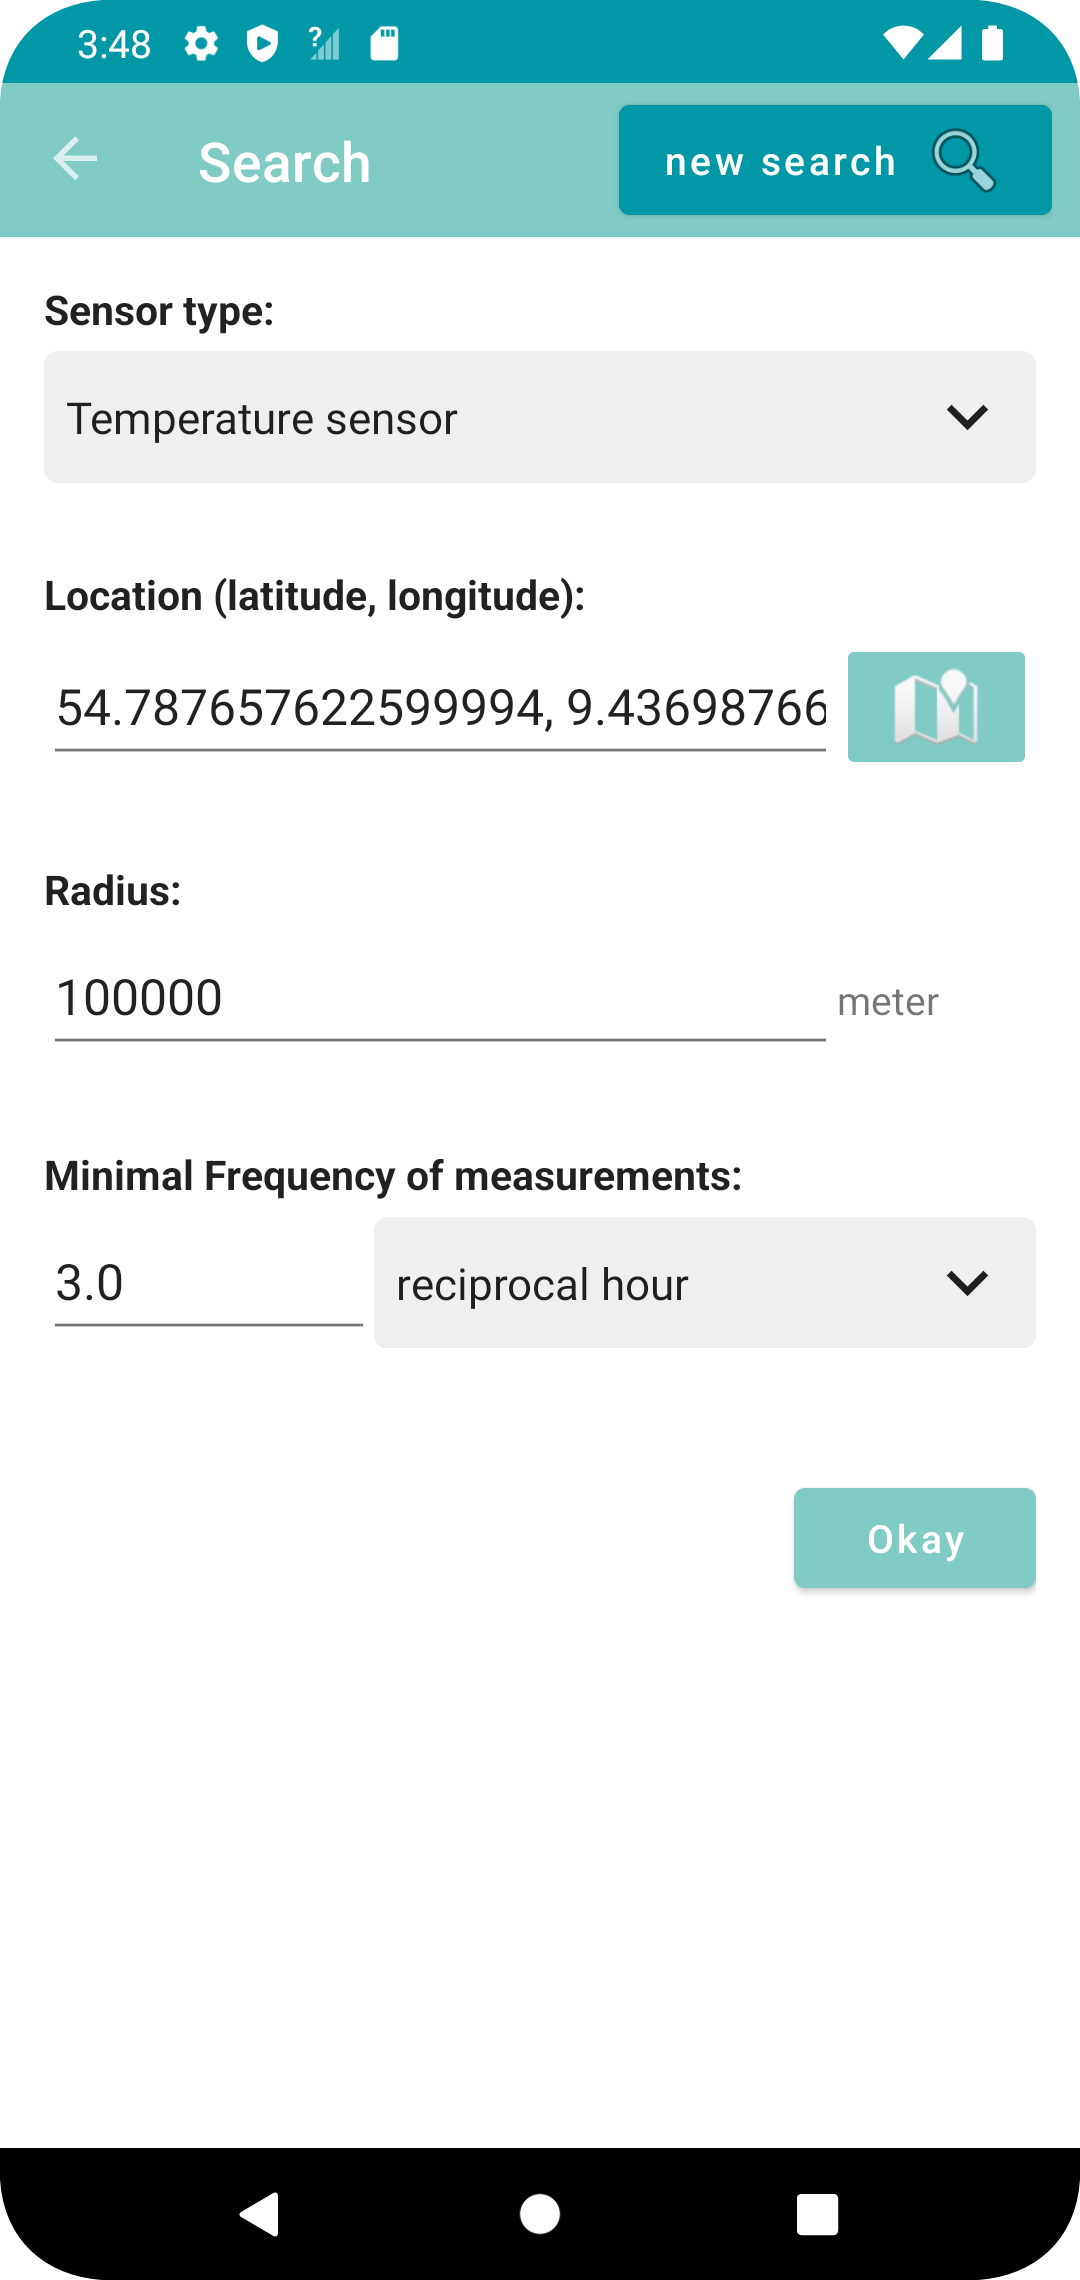
\includegraphics[scale=0.1]{screen_filter}
    \caption{Filter view}
    \label{fig:screen_main}
    \Description{
        The filter view offers the option to filter by sensor type, radius around a location, and minimum frequency of measured values. The location can be specified in longitude and latitude, or selected from a map. The unit for the frequency can be selected from a dropdown menu; the unit for the radius is meters.
    }
\end{figure}

In order to meet the requirements, we developed a filter view, which is shown in \autoref{fig:screen_main}. The view offers the option to filter by sensor type, radius around a location, and minimum frequency of measured values. The location can be specified in longitude and latitude, or selected from a map.

\begin{figure}[H]
    \centering
    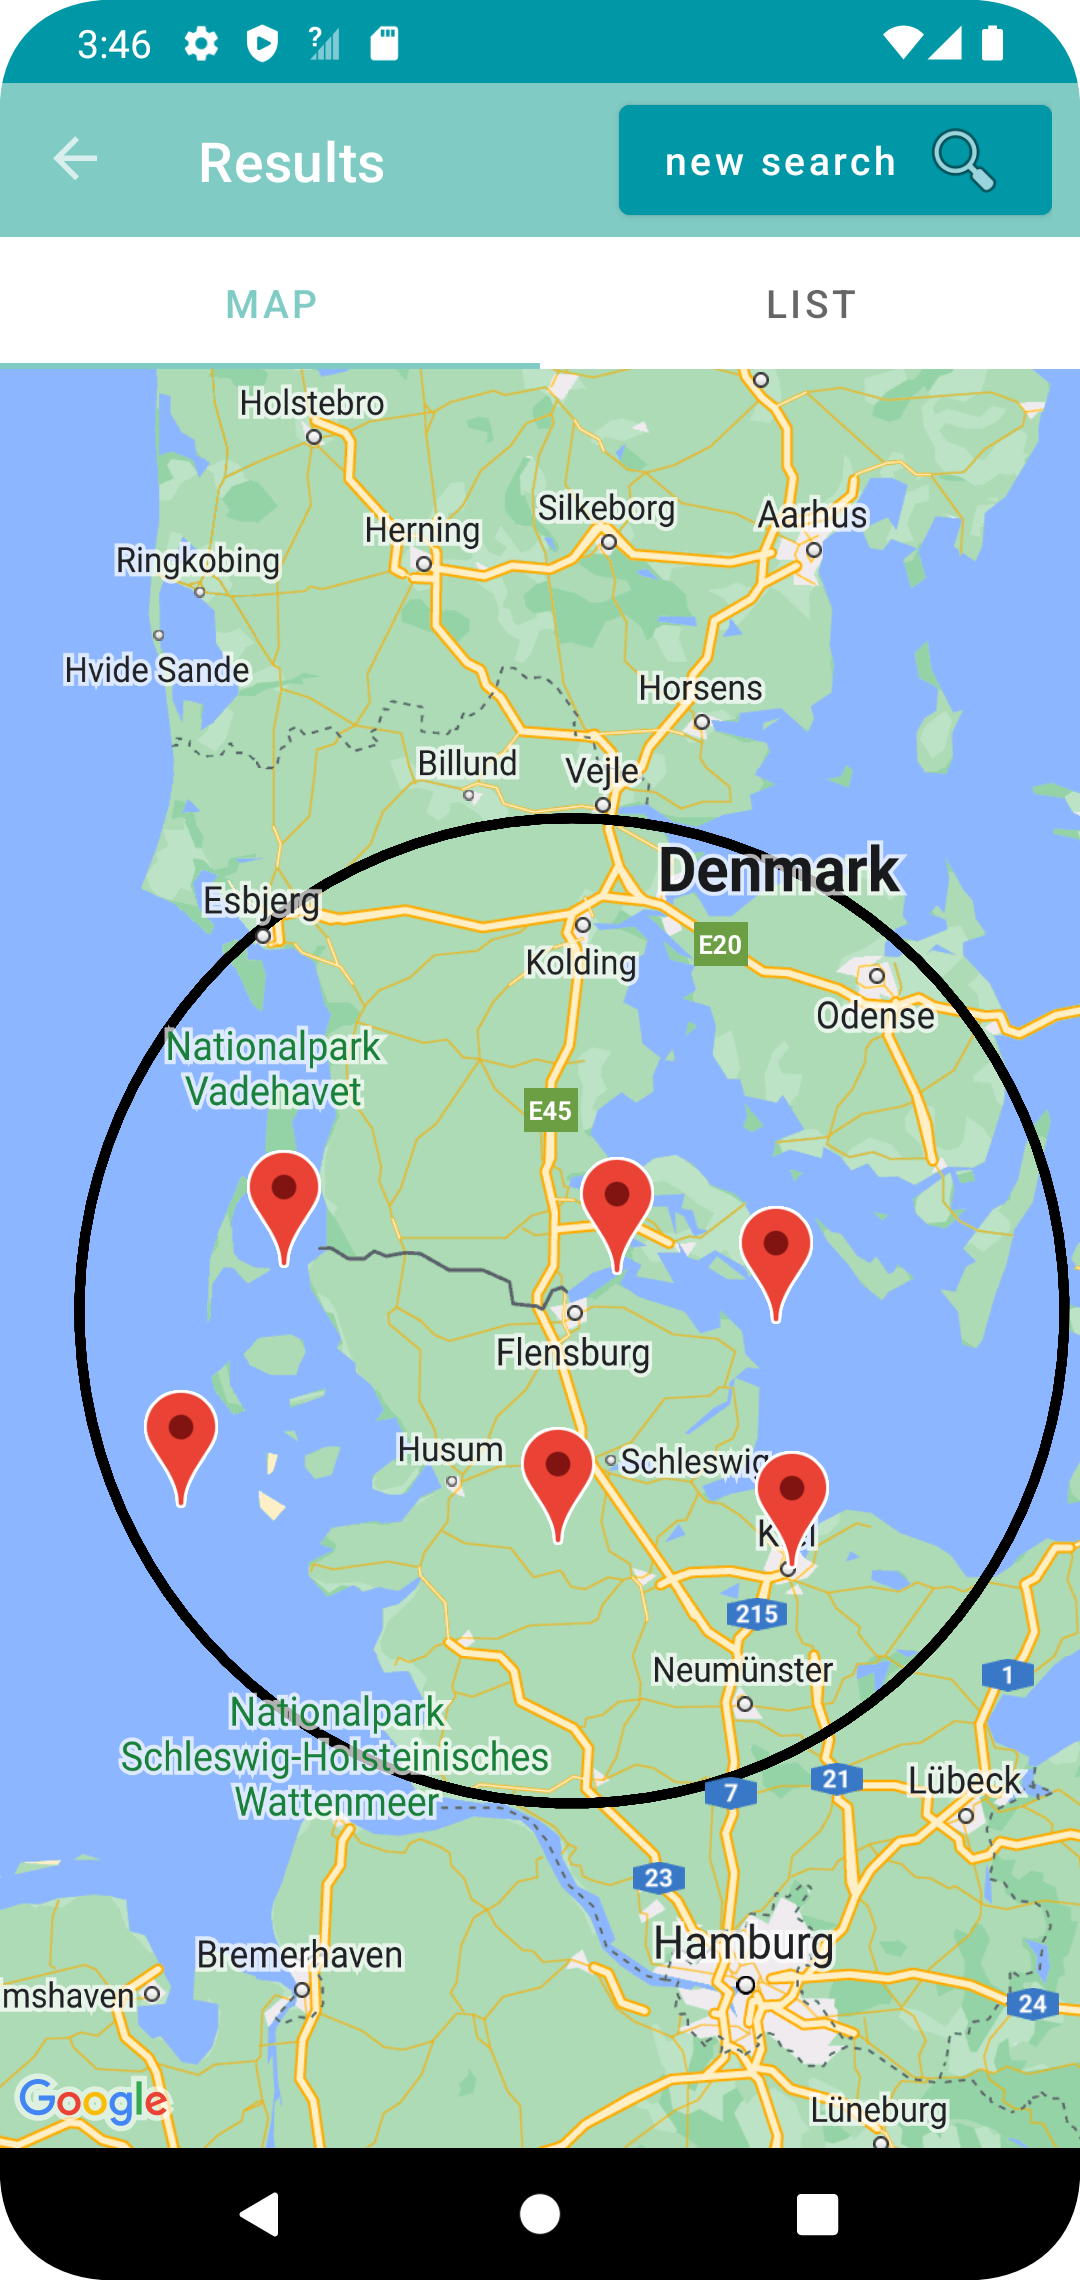
\includegraphics[scale=0.1]{screen_map}
    \caption{Map view showing the results}
    \label{fig:screen_results_map}
    \Description{
        The map view shows the sensors that match the filter criteria as well as a circle that represents the search area.
    }
\end{figure}

The sensors can be presented in a map or list view. This gives the user a quick overview of the surrounding sensors.

\begin{figure}[H]
    \centering
    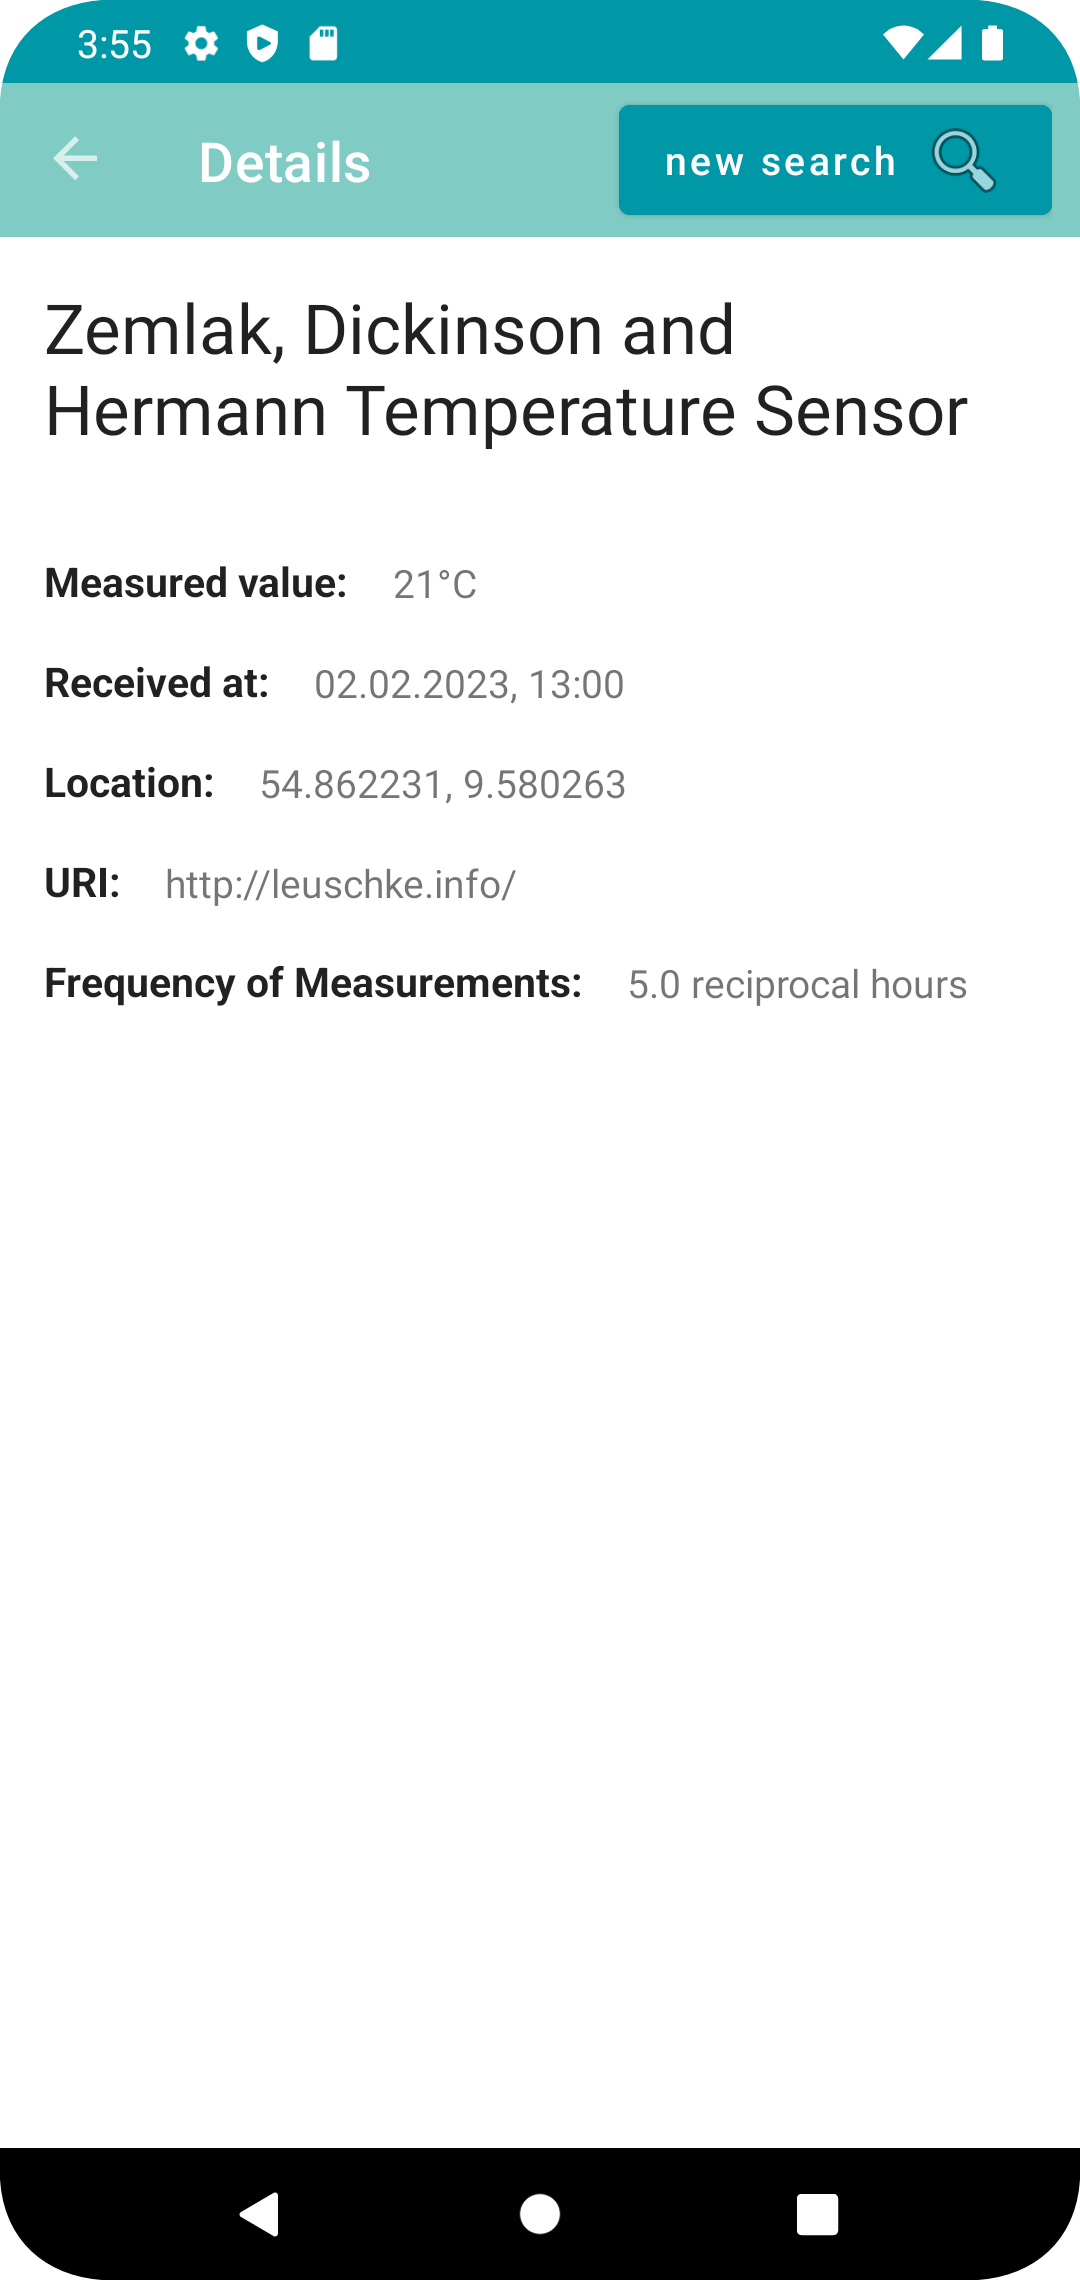
\includegraphics[scale=0.1]{screen_detail}
    \caption{Detail view of a sensor}
    \label{fig:screen_result_details}
    \Description{
        The detail view shows the metadata of the sensor and the most recent measured value.
    }
\end{figure}

The measured values and metadata will be displayed in a detailed view. It reads the data from the \gls{td} and presents them clearly to the user.

\subsubsection{JSON-LD}\label{sec:jsonld}

Since the server may hold heterogeneous data from different providers, the structure of \gls{jsonld} documents may vary, which prevents direct decoding. It first has to be normalized by expanding the data. Normalization with a different method, which could result in simpler data structures, may not work, because it could result in heterogeneous data. For example, multiple values for the same property would be encoded as an array, while a single value would be encoded as-is. Expansion would always result in an array of values, even if only a single value is present.


% TODO: App als Quelle verfügbar machen (für Veröffentlichung)

\subsection{Search}\label{sec:search}

As stated earlier, we used \emph{JSONPath} as the search option for our implementation to check whether \gls{wot} search is viable and advisable for use in open data contexts.

With \emph{JSONPath}, we cannot filter the \gls{tdd} by the exact filter options we have, since we cannot filter by a radius. We can only filter all \glspl{td} within a bounding box of the circle that would be the result of the radius. The filtering by the actual radius has to be done in a second step on the client side.

\autoref{lst:example-jsonpath-query} shows an exemplary \emph{JSONPath} query that would be used to search for all temperature sensors that are within the bounding box of the circle with a radius of 10 km around the specified center (54.8075525, 9.463745) and that have a minimum measurement frequency of 3 times per hour.

The actual query does not contain line breaks or indentation, but they have been added here for readability reasons. Some additionally required frequency measurement unit filters have been omitted for brevity as well.

\begin{lstlisting}[language=jsonpath,caption={Example JSONPath query},label={lst:example-jsonpath-query}]
$[*]?(
  @."geo:lat"<54.8973845209824
  &&
  @."geo:long"<9.6196146650183
  &&
  @."geo:lat">54.7177214790176
  &&
  @."geo:long">9.307875334981617
  &&
  @."@type"=="sdsc:TemperatureSensor"
  &&
  (
    (
      @."s4envi:hasFrequencyMeasurement"."saref:hasValue">=3.0
      &&
      @."s4envi:hasFrequencyMeasurement"."saref:isMeasuredIn"."@id"=="om18:reciprocal_hour"
    )
    ||
    (
      @."s4envi:hasFrequencyMeasurement"."saref:hasValue">=0.33333334
      &&
      @."s4envi:hasFrequencyMeasurement"."saref:isMeasuredIn"."@id"=="om18:hertz"
    )
    ||
    ...
  )
)
\end{lstlisting}


\section{Results}\label{sec:results}
% Backend/Frontend
In this study a reference implementation for working with sensors in a smart city was developed. It consists of a backend that is able to store and manage sensor information and a frontend in form of an android app to showcase the range of options of a \glsentrylong{tdd} and give a context to possible usage.

% WoT
The \gls{wot} is the only standardization in our area of work that enables interoperability. We found that it offers the required expressiveness and can be used for use cases similar to ours.
As a result, the data collected by providers and the data requested by users can be connected to each other in a clearer way using the \gls{wot}. The hardware and software requirements of the \gls{wot} can be easily met due to the fact that the \gls{wot} mainly works with technologies that are already widespread (e.g. \gls{http}, \gls{json}, \dots). The only downside we found is that the \gls{wot} does not include \glsxtrshort{qos} aspects. We solved this problem by creating an ontology with obligatory usage that does include them.

% Ontology
The ontology aligns with the \citetitle{w3c.wot.tdo.20230111} for specific use in \glspl{td}. It is well suited for our use case and can easily be altered to fit similar works to ours. Due to the uniform class hierarchy for each sensor type it is a straightforward process to extend the ontology to include more or different sensors. Additionally, we based our own ontology on well-established ones. These ontologies have been used in various different ontologies and projects, making it easier to compare our ontology to others and adjust existing ontologies based on our work.

%JSON-LD
One of the cruxes in our work was the \gls{jsonld} expansion and the handling of expanded data. In most cases, it is best to do this on the server side. There are however use cases where this is not sensible. Especially if the client gets data from multiple servers, it might be necessary to do the expansion on the client side to ensure that the data is parsed consistently. This would however also lead to a complex way of expanding the data. Regardless of where the expansion takes place, it can quickly become complex and there are not enough libraries for it to be easily usable on all typical platforms.

% Search
\emph{JSONPath} and thus syntactic searches are suitable for service discovery, but require that the \glspl{td} are normalized on the server side and that the type of normalization is known to consumers of that \gls{tdd}. For consistency, the normalization should be done using expansion. Difficulties can arise when a property used for filtering can be specified in different units, since all possible units have to be provided a filter for. This complicates the filtering process and makes it more prone to errors. In addition, since multiple servers may use different normalization strategies, queries would not be universally usable. Semantic search, in contrast, is harder to implement, but easier to use, since it does not require normalization, which aligns more with the idea of \gls{jsonld} that has been outlined before. In both cases, client-side normalization is strongly recommended, if not required.

% Integration in bestehende Systeme
\glsentrylongpl{td} for \glsentrylong{sd} itself is an important step and more work needs to be done be able to use it. Through the usage of ontologies, all data about the sensors is provided in a uniform format. However, when requesting data from a specific sensor the format still depends on the sensor itself.

\section{Conclusion}\label{sec:conclusion}

We implemented a reference of how to serve \glspl{td} and the variety of search options in a \gls{wot} context. A mobile application was used to show realistic use cases.

The lack of a standard ontology for Smart City contexts in the \gls{wot} specification has been solved by creating a new ontology based on established ontologies. It has been designed for easy extension of missing sensor types and the integration of search-relevant \gls{qos} aspects.

Despite the missing ontology, the proven expressiveness of and widespread availability of required hard- and software for the \gls{wot} suits \gls{sd} in open data contexts, providing a unifying concept for making different data endpoints available to a variety of users.

The usage of \gls{jsonld} throughout the \gls{wot} imposes normalization and verbosity difficulties on both servers and clients, especially if syntactic search methods are used, due to the possible heterogeneity of multiple \glspl{td}.


% \listoffigures
% \listoftables
\printglossaries{}
\printbibliography[heading=bibintoc]

% \appendix
% \input{sections/A-ontology-definitions}

\end{document}
